\chapter{Experiments} \label{ch:experiments}
In this Chapter we will explore different scenarios obtained by changing parameters, number of population agents and we will try to maximize the Revenue as the KPI of the system. For the note, comments see the Chapter \ref{ch:conclusion}.
\subsection{Original setup}
From the simulation panel I setup the simulation duration to 960 minutes that correspond to 16 hours. The initial population are:
\begin{itemize}
\item 20 Worker\_iron
\item 15 Buyer
\item 10 Rider
\end{itemize}
Then the other parameters:
\begin{itemize}
\item perc\_revenue : 0.15\%
\item fixed\_cost :0.20€
\item workerArrRate: 20 per hour
\item buyerArrRate: 20 per hour
\item riderArrRate: 10 per day
\item Cost: 64€ per day each rider
\end{itemize}
Here the results:
\begin{figure}[hbtp]
\caption{Original setup simulation}
\centering
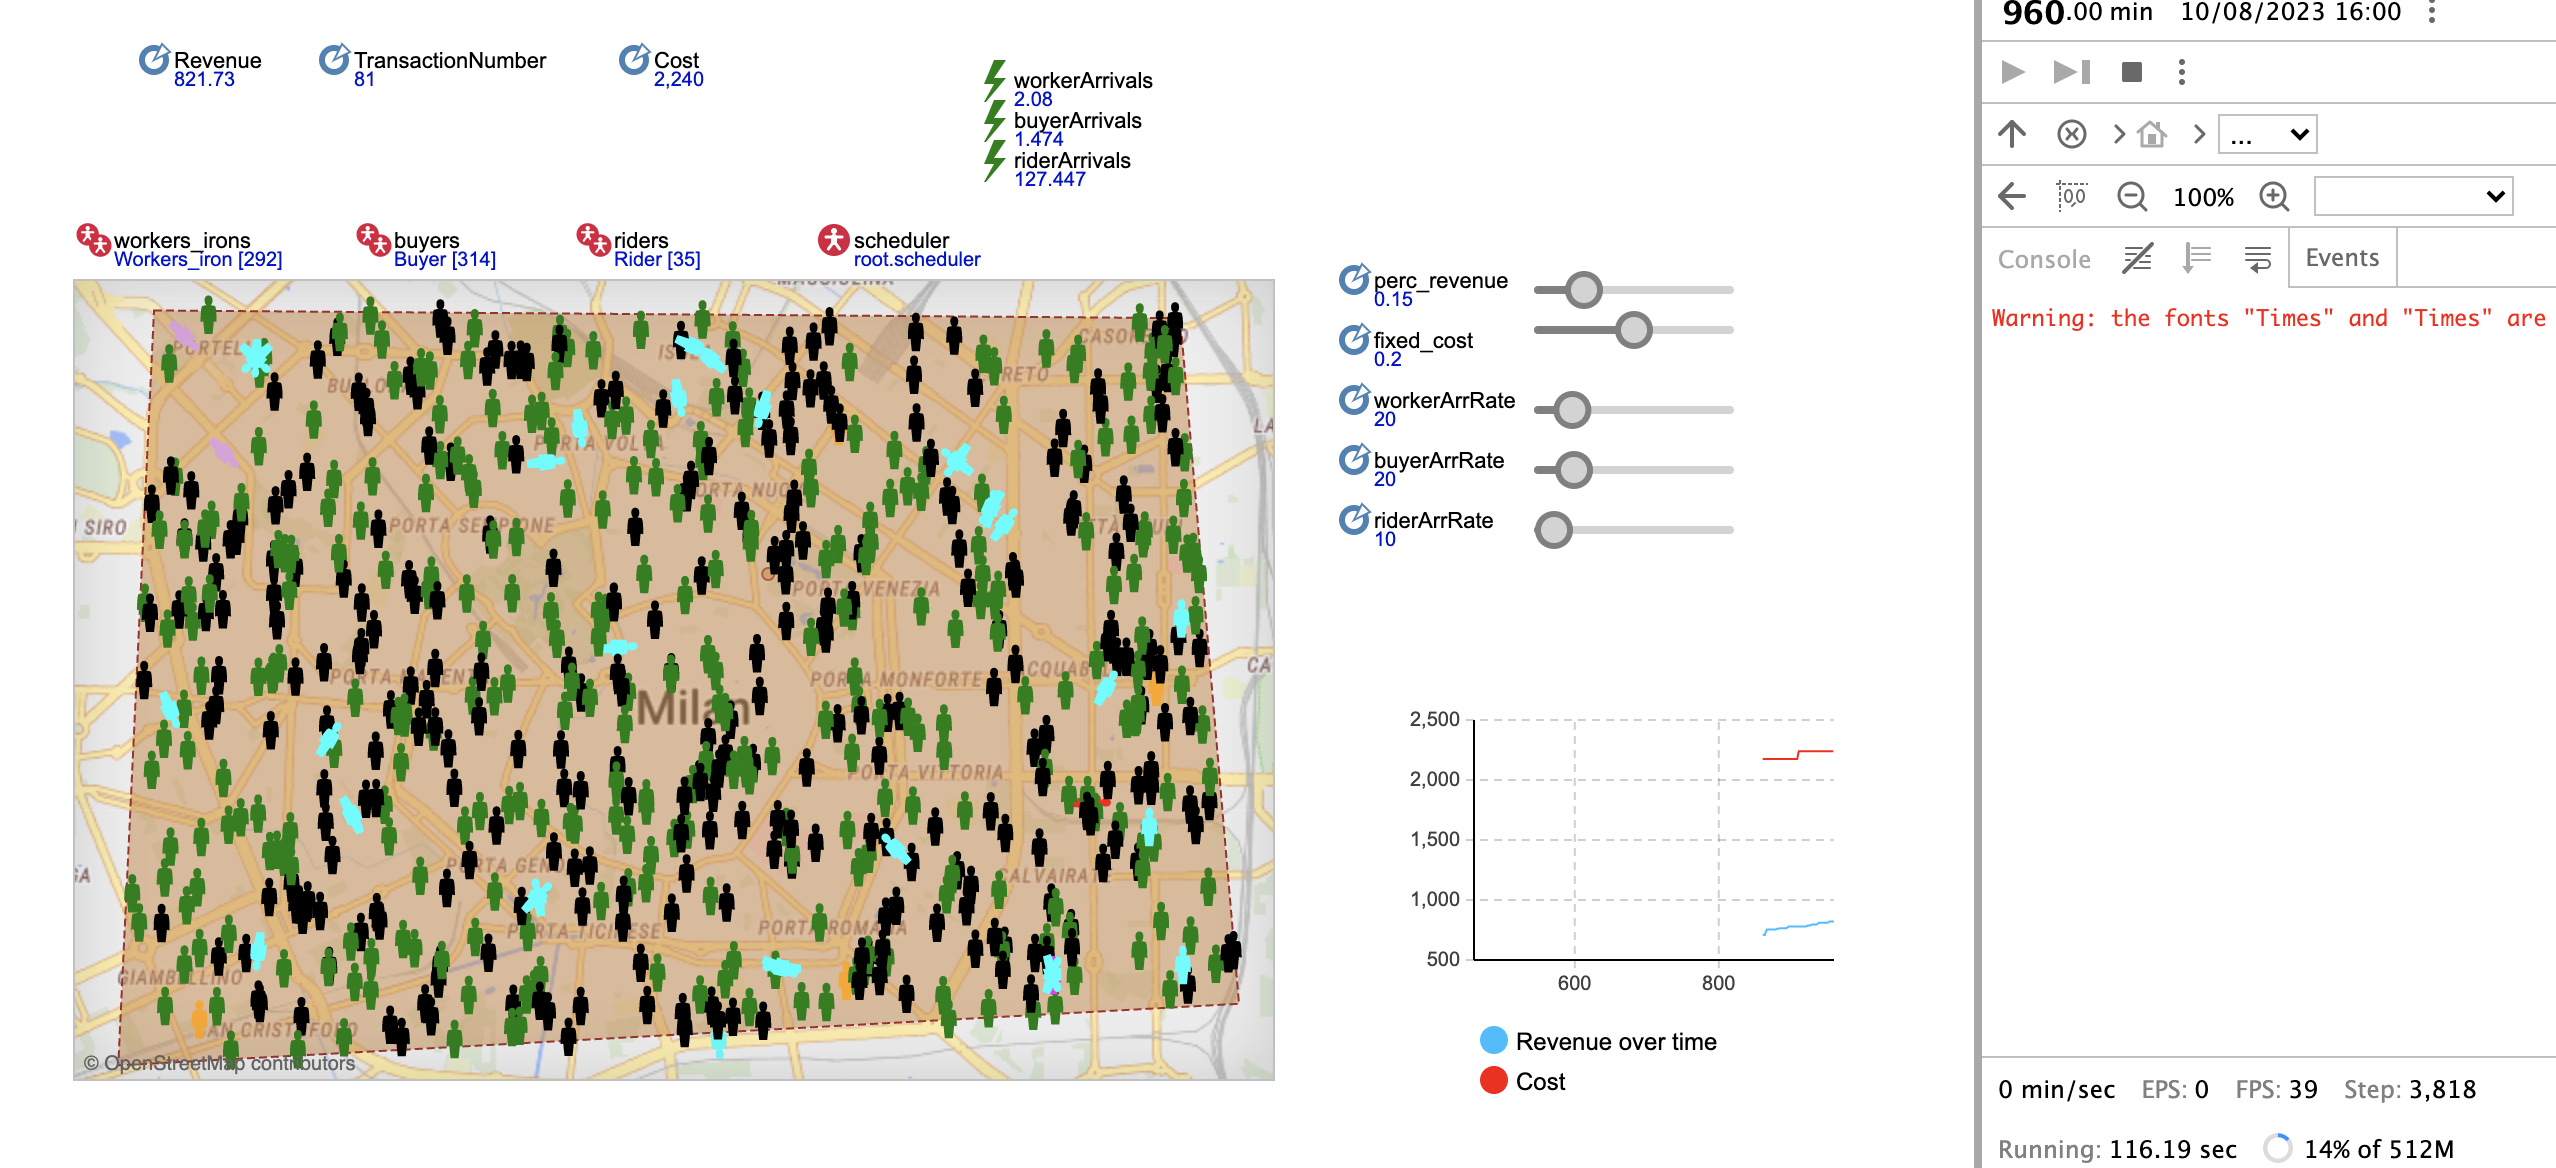
\includegraphics[scale=0.3]{../Images/sim01.png}
\end{figure}
As you can see from the top KPI or form the chart in the bottom-right side the Revenue are below the Cost. So there will be a lost over the first day. So we need to change some parameters and check if the situation will be better or not. For doing that I applied the What-If scenario different time as reported below.
\subsection{What-If scenario 1: Same configuration - lower rider cost}
By just reducing the cost of the rider we can obtain a profit, with the same parameters. Of course this is not the optimal way. Indeed there are national law that ensure the right price for each worker, in this case the rider. However here the simulation image:
\begin{figure}[hbtp]
 \caption{Lower price for rider}
 \centering
 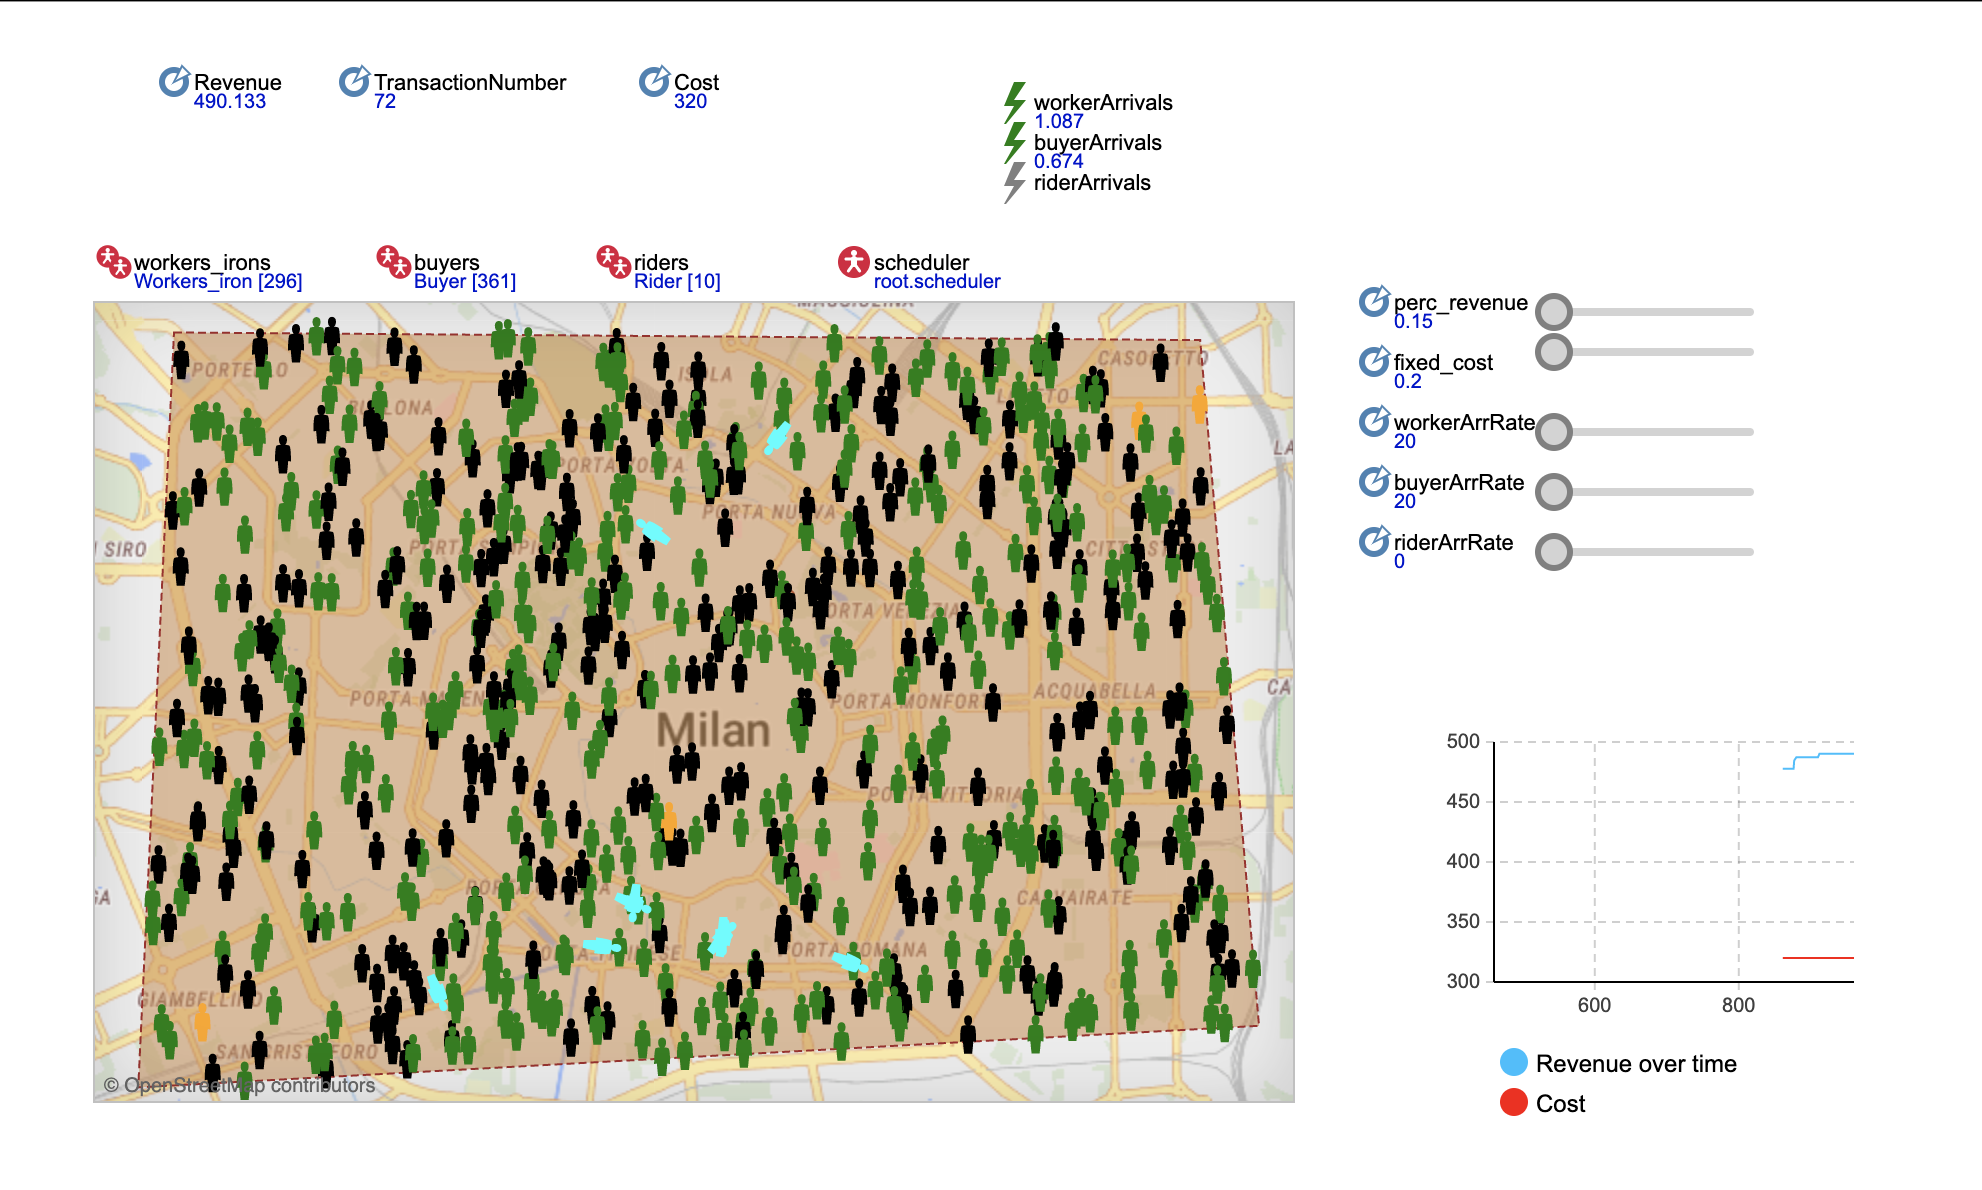
\includegraphics[scale=0.3]{../Images/sim03.png}
 \end{figure}
\subsection{What-If scenario 2: Increasing earning parameters}
Configuration setup:
\begin{itemize}
\item perc\_revenue : 0.3\%
\item fixed\_cost :0.30€
\item workerArrRate: 20 per hour
\item buyerArrRate: 20 per hour
\item riderArrRate: 0 per day
\item Cost: 64€ per day each rider
\end{itemize}
Here the result:
\begin{figure}[hbtp]
\caption{Increasing earning params simulation}
\centering
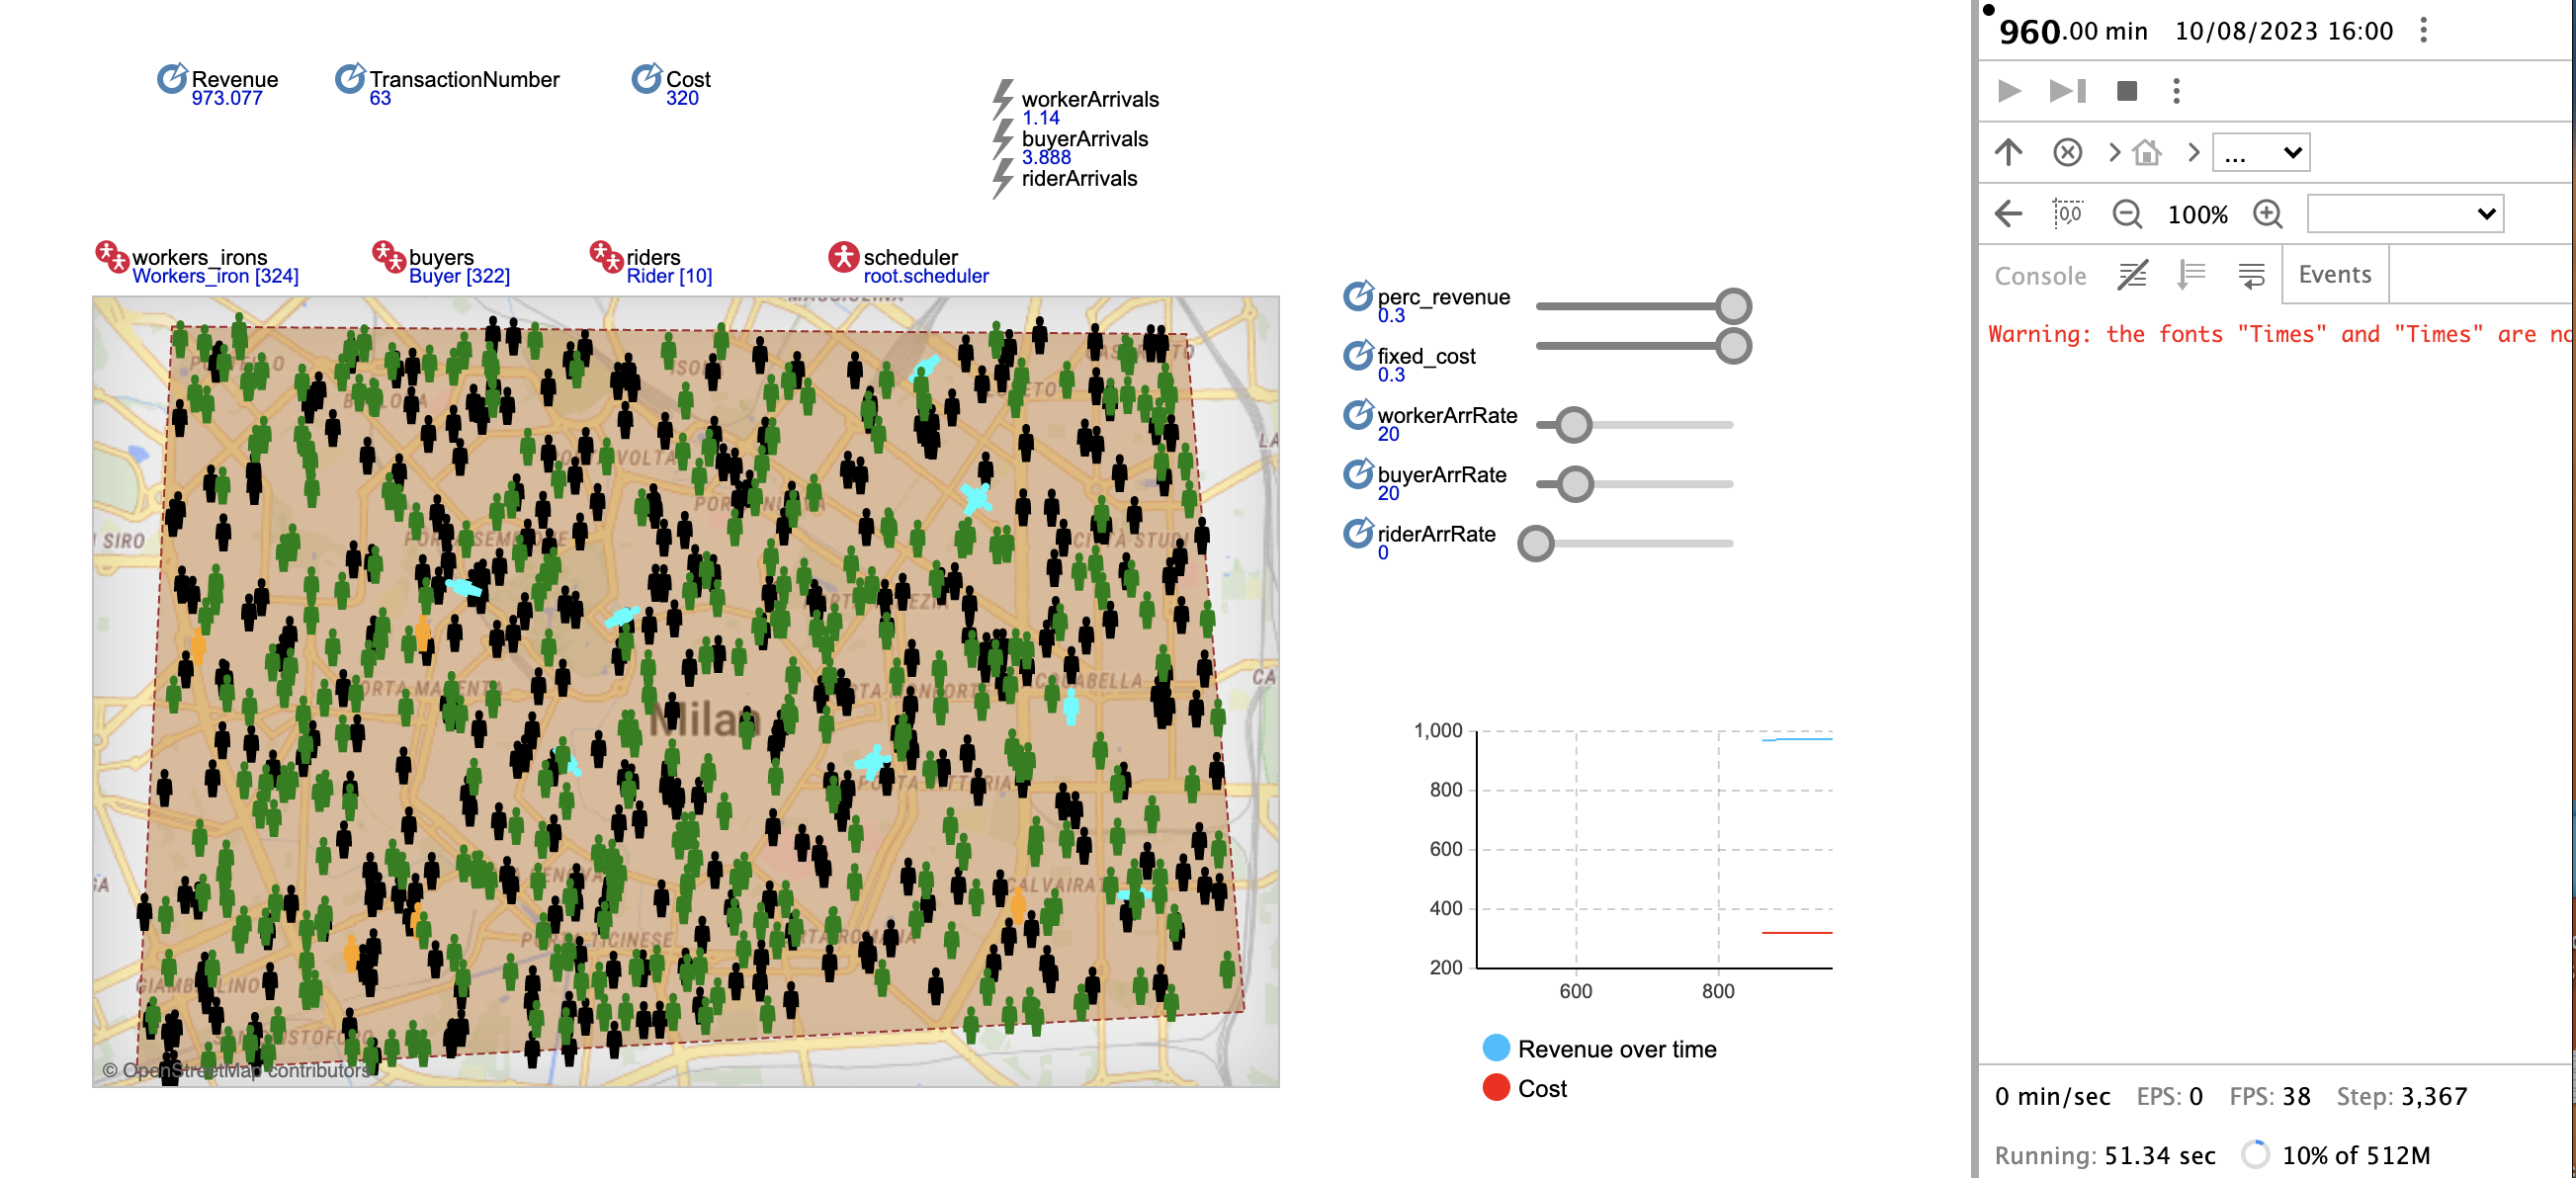
\includegraphics[scale=0.3]{../Images/sim04.png}
\end{figure}
\subsection{What-If scenario 3: Increasing rider speed}
Originally, the rider speed was set to 10 km/h. By increasing this number to 50 km/h the percentage of valid transaction is 52\% more then the previous experiment. Then, for this experiment, the initial number of riders are 100. 
The result are shown in Figure \ref{figure:sim05}.
\begin{figure}[hbtp]
\caption{Increasing  rider speed simulation}
\label{figure:sim05}
\centering
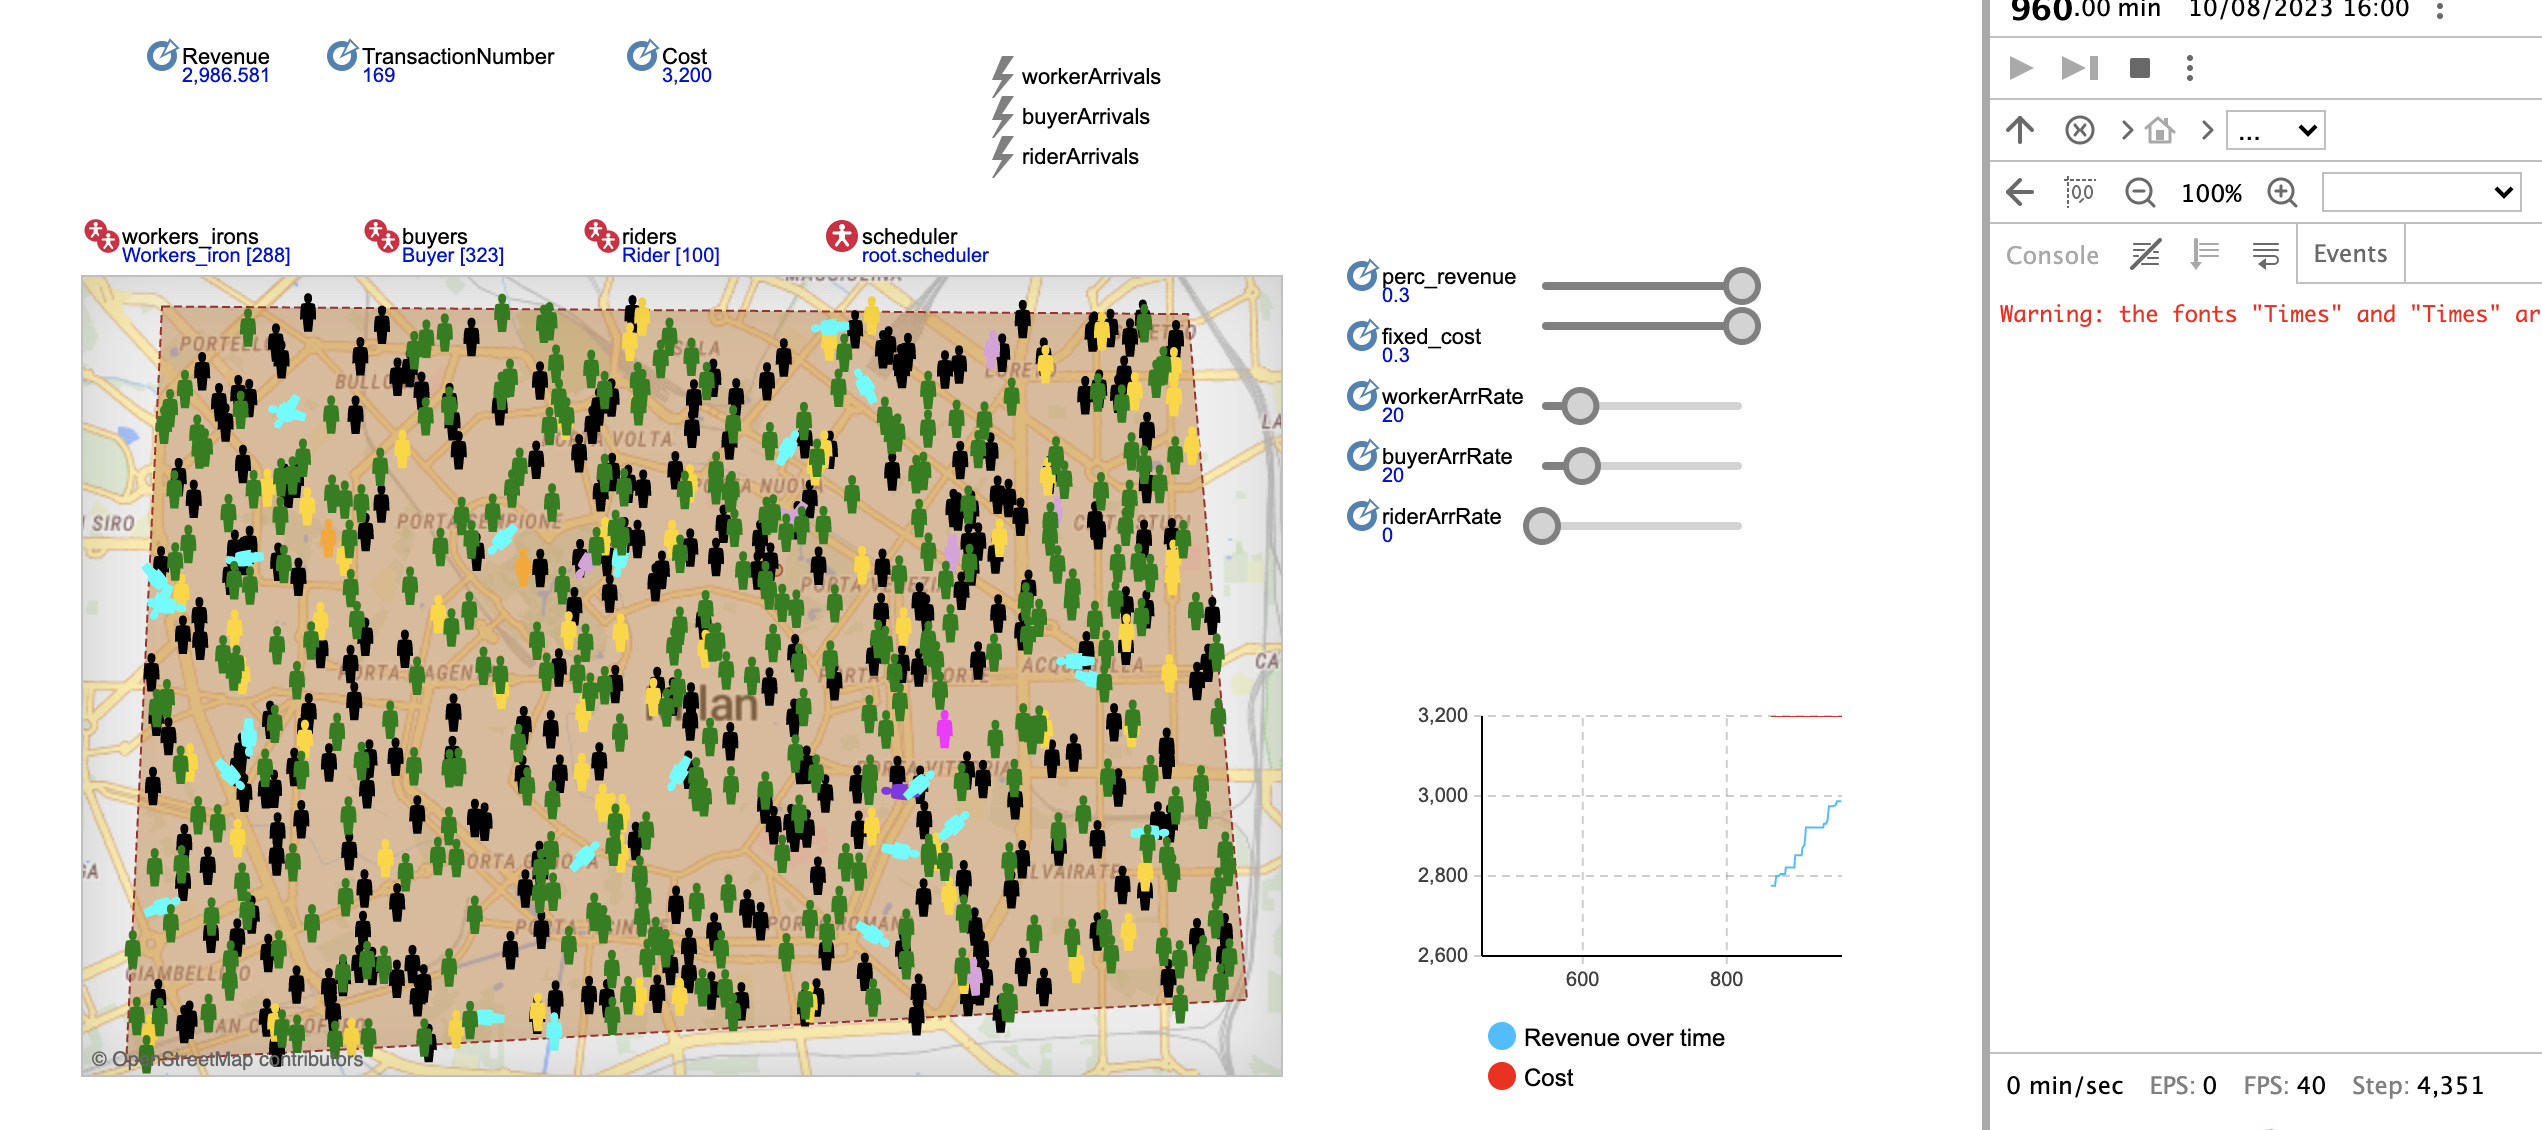
\includegraphics[scale=0.3]{../Images/sim05.png}
\end{figure}
\subsection{What-If scenario 4: Increasing worker and buyer rate (50 per hour)}
By increasing the number of order and the number of worker to 50 per hour we obtain 4200€ as Revenue with 276 valid transaction. The cost still remain 3200 considering 100 rider as amount of population. 
The result are shown in Figure \ref{figure:sim06}.
\begin{figure}[hbtp]
\caption{Increasing number of worker/buyer per hour }
\centering
\label{figure:sim06}
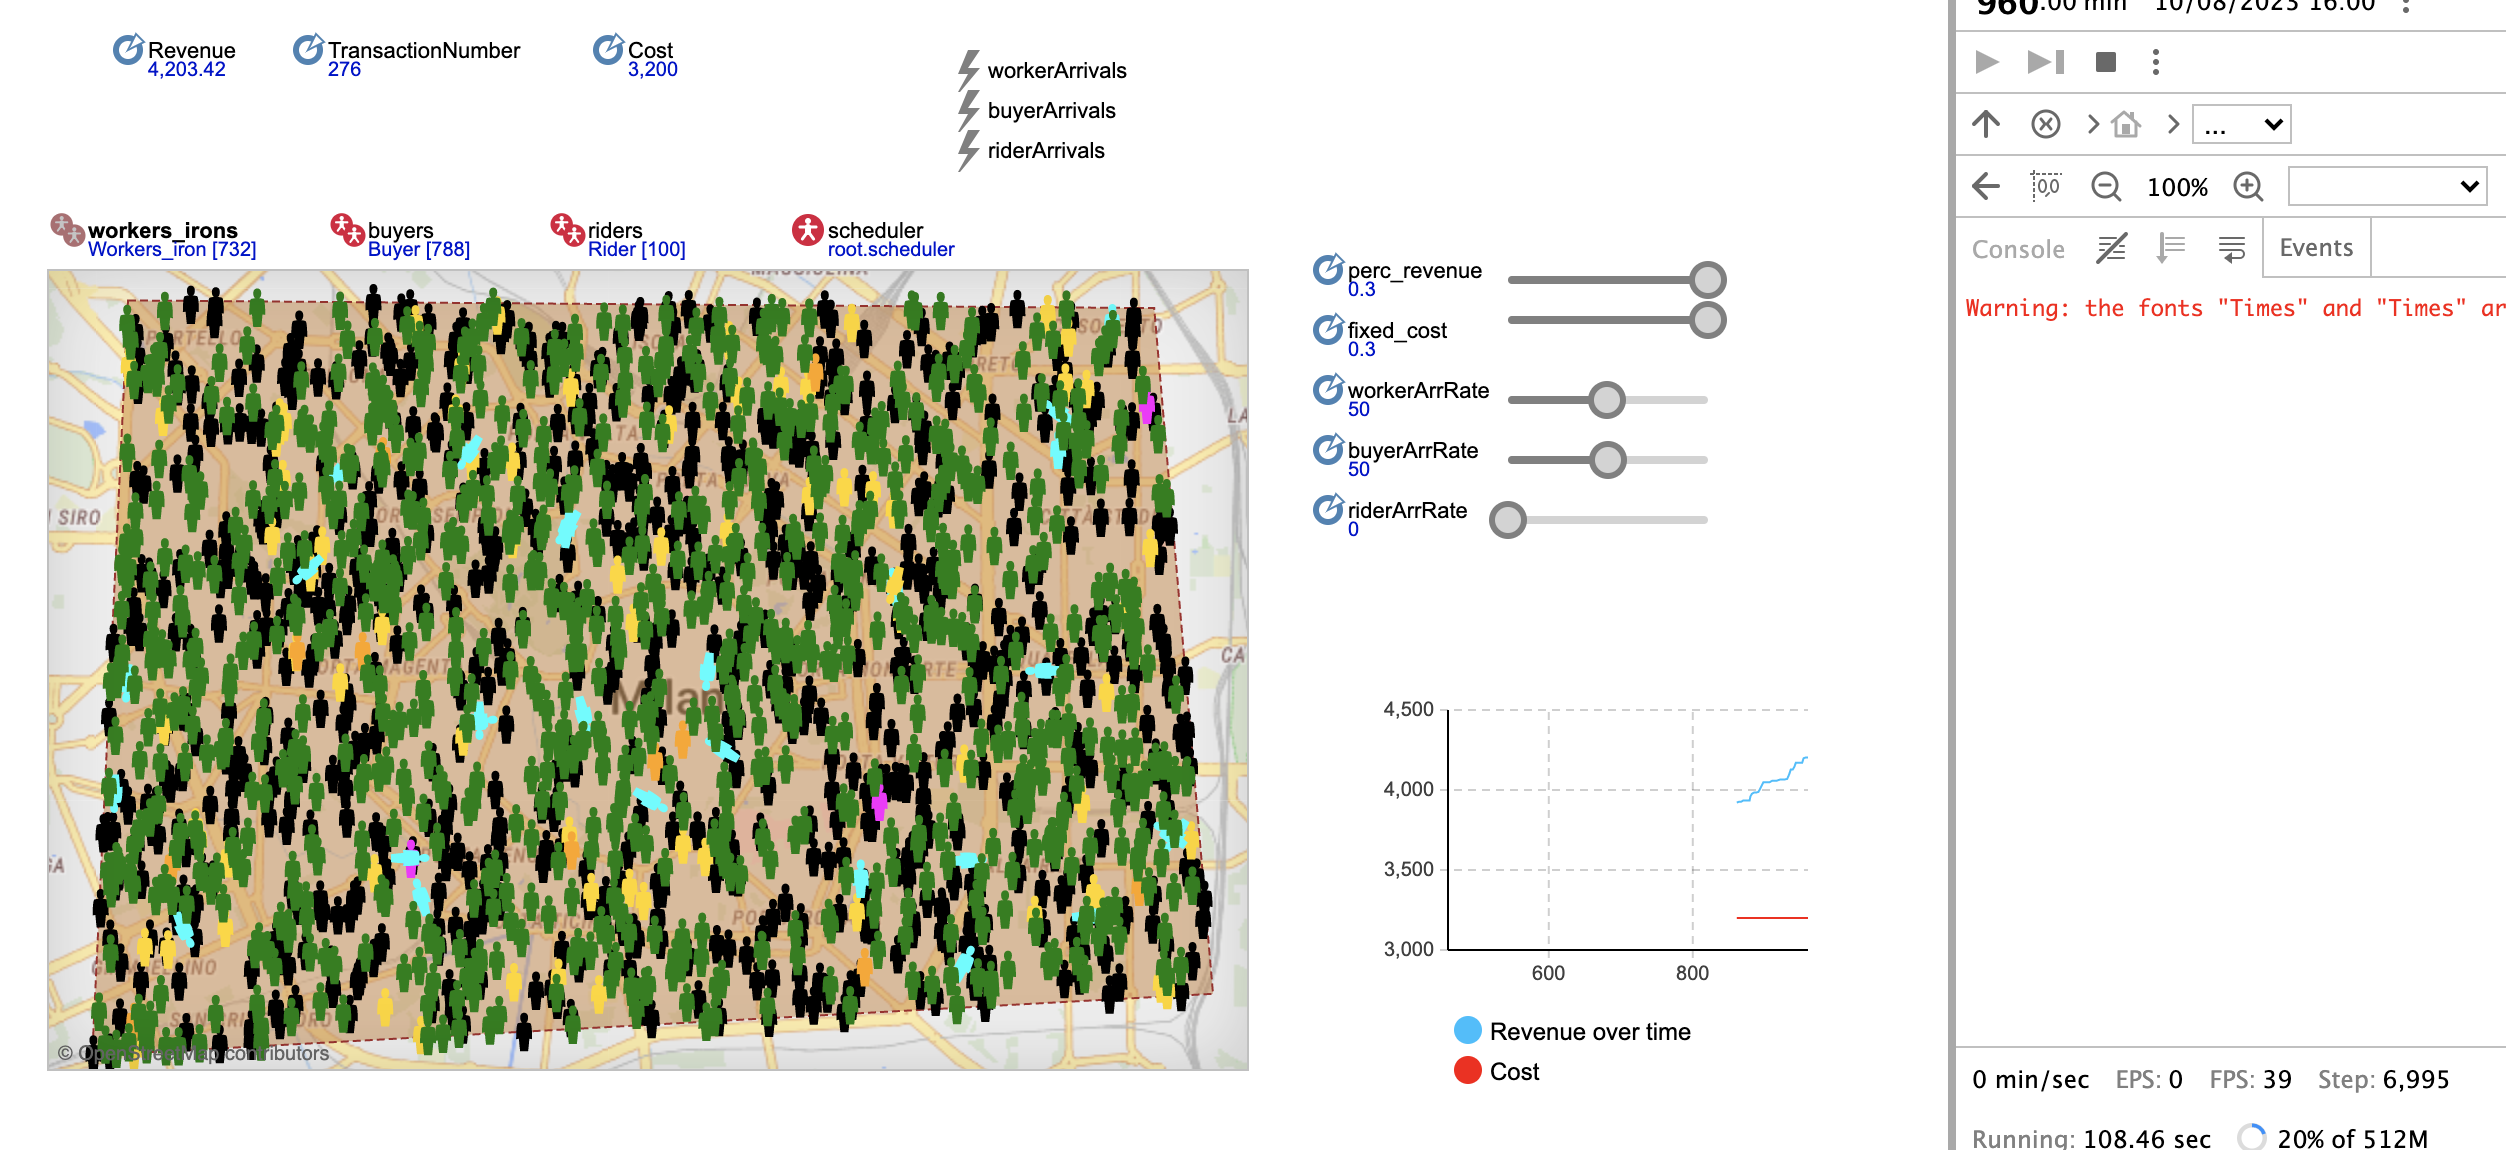
\includegraphics[scale=0.3]{../Images/sim06.png}
\end{figure}
